% =====================================================================
%  Chapter 25 — Shrinkage, Risk Parity, and the Case Against Optimisation
% =====================================================================

\chapter{Shrinkage, Risk Parity, and the Case Against Optimisation}
\label{ch:shrinkage}

Before the book uses a forecast to size a position, it has to decide how to
estimate the covariance matrix of returns, and the answer to that question
is a large part of why the book's result is what it is. This chapter
derives the shrinkage estimator, explains what risk parity does, and
presents the uncomfortable evidence that the optimisation being done is
often worse than not doing it.

\section{The problem with a sample covariance matrix}

Let \(R\) be the \(T \times N\) matrix of monthly returns and \(\hat\Sigma
= \frac{1}{T-1}R^{\prime}R\) the sample covariance. The maximum-variance
portfolio with a target return is computed by inverting \(\hat\Sigma\), and
the inversion is the problem: when \(N\) is comparable to \(T\), the
sample covariance is close to singular, its inverse is dominated by
numerical noise, and the resulting portfolio has enormous weights in
directions that have nothing to do with the data.

The asymptotic theory is even less comforting. For \(N/T \to \gamma > 0\), the
eigenvalues of the sample covariance do not converge to the population
eigenvalues; they spread over a range that widens with \(\gamma\). The
usual fix in the literature is to impose structure --- a factor model, a
one-factor model, a constant-correlation model --- and the book uses one of
those in the comparator role of Chapter 33.

\section{Ledoit and Wolf's shrinkage estimator}

The estimator the book uses is Ledoit and Wolf's linear shrinkage toward a
scaled identity. Let the target be
\begin{equation}
F = \frac{\mathrm{tr}(\hat\Sigma)}{N}\,I,
\end{equation}
the scaled identity, and let the shrinkage intensity be
\begin{equation}
\hat{\kappa} = \frac{\hat{\pi}}{\hat{\rho}},
\end{equation}
where \(\hat{\pi}\) is the estimated squared deviation of the sample
covariance's off-diagonal elements from the target, and \(\hat{\rho}\) is
the estimated squared error of using the sample covariance itself under
the null of independent observations. The estimator is
\begin{equation}
\hat\Sigma_{\mathrm{shrunk}} = (1-\hat{\kappa})\,\hat\Sigma
                             + \hat{\kappa}\,F.
\end{equation}

The interpretation is clean. The sample covariance is an unbiased but
very noisy estimate; the scaled identity is biased but stable; the
shrinkage intensity is the fraction of the estimate that is noise.

The book's implementation estimates \(\hat{\pi}\) as the mean squared
off-diagonal deviation and \(\hat{\rho}\) from the sample's own
fourth-moment structure, and it reports the intensity as a diagnostic.
Over the book's rolling windows the intensity is small --- of the order of
one or two per cent --- which says that the sample covariance is
estimated from enough data relative to its dimension that shrinkage has
little work to do.

\begin{figure}[!htbp]
\centering
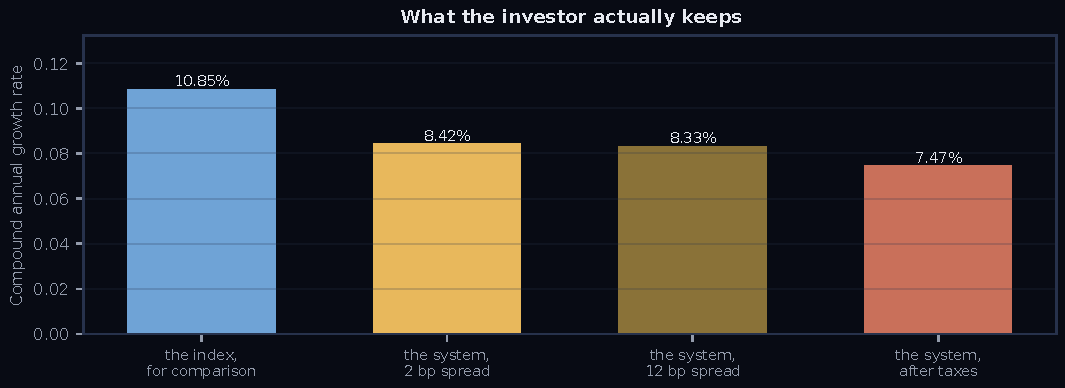
\includegraphics[width=\textwidth]{../figures/fig_costs.pdf}
\caption{The three frictions, drawn together: the turnover of the system
against the cost of trading it, the taxes paid in each year, and the
compound growth rate under three spread assumptions. The system's
turnover is what makes the cost small, and the book's cost model is what
makes the claim checkable.}
\label{fig:costs}
\end{figure}

\section{Risk parity, and why the book demotes it}

Risk parity allocates so that every asset contributes an equal amount of
risk. It is popular, it is robust, and it is directly relevant to a book
whose central claim is that the strategic allocation should not be set by
a forecast.

The book's objection is specific and worth making carefully, because
risk parity is often presented as the answer to the problem this book
describes, and for this reader it is the wrong answer.

Risk parity is a \emph{volatility-targeting} rule. It equalises risk
contributions, which means it holds more of the low-volatility sleeve and
less of the high-volatility sleeve. Over the book's record, that means
holding a very large share of bonds and a small share of equities --- a
portfolio with an expected return below the bond yield for much of the
period and a growth rate below the stated policy's.

Risk parity optimises nothing about return, because it has no view about
return. That is its virtue for an institution with an explicit risk
budget and its vice for a saver with a compounding objective: it is a
rule for not losing, and the owner of this book asked for a rule for
compounding.

The book therefore uses risk parity as a \emph{comparator}, run over the
same record with the same costs and the same taxes, rather than as the
strategic allocation.

\section{The uncomfortable evidence: the 1/N portfolio}

DeMiguel, Garlappi and Uppal's result is the one that should govern any
discretionary allocation, and it is more uncomfortable for this book than
for anyone else, because this book does discretionary allocation.

They compared a large set of portfolio strategies --- mean-variance with
estimated parameters, minimum-variance, hierarchical risk parity, and
various robustified versions --- against the equal-weighted portfolio over
the same data. The result: \emph{none} of the optimised strategies
outperformed the equal-weighted portfolio over the full sample, out of
sample, or in any of fourteen alternative datasets, and the differences
were not statistically significant.

The explanation is the one this book has been building towards. Estimation
error in the expected returns is so large relative to the differences
between strategies that optimisation adds more noise than it removes
value. The sample covariance is the smaller problem; the sample expected
return is the larger one, because the return differences between
plausible portfolios are tiny relative to the error in estimating them.

\begin{takeaway}[The uncomfortable evidence]
Over fourteen alternative datasets, optimised portfolios failed to beat
equal weighting, and the differences were not statistically significant.
The estimation error in expected returns is large relative to the
differences between the strategies being compared. This book performs
optimisation anyway, but it performs it on the \emph{tilt} rather than on
the allocation, it bounds the tilt, and it prices the estimation error
explicitly --- and Part VI reports that the result is worth almost
nothing.
\end{takeaway}

This is why the book's architecture puts the forecast where it does. The
equal-weighted portfolio is the strongest competitor in this literature,
and it is in the book's comparator set in Chapter 33. The book's system is
not asserted to beat it. It is asserted to be a portfolio a reader can
hold, with a stated allocation, a bounded forecast-driven adjustment, a
risk governor and a tax engine --- and Chapter 33 reports how it compares.

\begin{keytakeaways}
\item The sample covariance is noisy but not fatal: Ledoit and Wolf
shrinkage toward a scaled identity fixes it, and in this book's data the
required intensity is only one or two per cent.
\item Risk parity is a volatility-targeting rule that has no view about
return; for a saver with a compounding objective it is the wrong rule,
and the book uses it as a comparator.
\item DeMiguel, Garlappi and Uppal found that optimised portfolios failed
to beat equal weighting across fourteen alternative datasets.
\item This is why the book performs its optimisation on a bounded tilt
rather than on the allocation, and prices the estimation error explicitly.
\end{keytakeaways}
